\documentclass{article}

\title{Sortowanie plików sekwencyjnych}
\author{Dominik Lau (188697)}

\usepackage{blindtext}
\usepackage{amsmath}
\usepackage[utf8]{inputenc}
\usepackage[polish]{babel}
\usepackage[T1]{fontenc}
\usepackage{listings}
\usepackage{color}
\usepackage{amssymb}
\usepackage{esvect}
\usepackage{graphicx}
\usepackage{mathtools}
\usepackage[margin=0.5in]{geometry}
\DeclarePairedDelimiter\ceil{\lceil}{\rceil}
\DeclarePairedDelimiter\floor{\lfloor}{\rfloor}

\graphicspath{ {./obrazy/} }

\definecolor{dkgreen}{rgb}{0,0.6,0}
\definecolor{gray}{rgb}{0.5,0.5,0.5}
\definecolor{mauve}{rgb}{0.58,0,0.82}
\def\multiset#1#2{\ensuremath{\left(\kern-.3em\left(\genfrac{}{}{0pt}{}{#1}{#2}\right)\kern-.3em\right)}}

\lstset{frame=tb,
  language=C++,
  aboveskip=3mm,
  belowskip=3mm,
  showstringspaces=false,
  columns=flexible,
  basicstyle={\small\ttfamily},
  numbers=none,
  numberstyle=\tiny\color{gray},
  keywordstyle=\color{blue},
  commentstyle=\color{dkgreen},
  stringstyle=\color{mauve},
  breaklines=true,
  breakatwhitespace=true,
  tabsize=3
}


\begin{document}
\maketitle

\section{Wprowadzenie}
Do zaimplementowania wybrałem algorytm sortowania przez scalanie w schemacie 2+1 (czyli z użyciem trzech taśm).  
Wylosowane przeze mnie typy rekordów to \textbf{numery rejestracyjne samochodów}, które miałem uporządkować \textbf{leksykograficznie}. Implementacji dokonałem w 
języku C++,  przyjąłem rozmiar rekordu $R=7$ [B], najpierw jako rozmiar strony ustaliłem  $B=70$ [B] a następnie
$B=700$ [B].
\section{Sortowanie przez scalanie}
Sortowanie to składa się z kolejnych iteracji (faz), z czego każda faza ma dwie części. Oto pseudokod
\begin{lstlisting}
while(!sorted){
	[tape1, tape2] = distribute(tape)
	[tape,  sorted] = merge(tape1, tape2)
}
\end{lstlisting}
\textbf{Dystrybucja} polega na rozkładaniu kolejnych ciągów niemalejących (serii) wartości w taśmie wejściowej 
na zmianę na dwie taśmy pomocnicze.  \textbf{Scalanie} to łączenie kolejnych serii i zapisywanie ich na taśmie. 
W ten sposób z każdą iteracją w sortowanej taśmie powstaje coraz więcej serii aż do momentu powstania pojedynczej. Wówczas plik jest posortowany. \\\\
Algorytm ten pozwala na posortowanie
danych o rozmiarze większym niż rozmiar pamięci operacyjnej. W wypadku tego algorytmu zużywamy 
\begin{gather*}
	S_{\text{DYSK}} = NR \text{  [B]}\\
	S_{\text{RAM}} = B \text{  [B]}
\end{gather*}
gdzie $B$ - rozmiar strony (bloku) pamięci w bajtach, $N$ - ilość rekordów, $R$ - rozmiar rekordów w bajtach. Warto zwrócić uwagę, że 
\begin{gather*}
	S_{\text{RAM}} = O(1)
\end{gather*}
Oto statystyki prezentowanego algorytmu
\begin{gather*}
	T_{\text{Pes}} = \frac{4N\ceil{log_2(N)}}{b} \text{  [i/o]}\\
	T_{\text{Avg}} = \frac{4N\ceil{log_2(N) - 1}}{b} \text{  [i/o]}
\end{gather*}
gdzie $b = \frac{B}{R}$, pozostałe oznaczenia jak powyżej.  Czas wykonania algorytmu liczony jest w ilości operacji
dyskowych.
\section{Specyfikacja pliku}
\subsection{Szczegóły implementacyjne}
Plik sekwencyjny w kodzie reprezentuje klasa \textit{Tape}, która jest generyczna i może być rozszerzona na inne typy rekordów. W ramach publicznego
interfejsu udostępnia ona metody do odczytu aktualnego rekordu, pobrania następnego rekordu (w trybie odczytu) oraz dodawania rekordu (w trybie zapisu).
Szablonowa klasa bazowa rekordu zdefiniowana jest w pliku \textit{RecordIfc.h}.  
Folder \textit{impl} zawiera implementację wyżej wymienionych interfejsów
do rekordu numeru rejestracyjnego.  Klasa rekordu udostępnia operacje \textbf{serializacji i deserializacji} oraz porównywania.
\subsection{Zapis}
Bloki z taśmy są zapisywane bezpośrednio do pliku po wcześniejszej serializacji rekordów. \textbf{Serializacja rekordów} polega na przedstawieniu 
znaków wchodzących w skład numeru rejestracji w formie siedmiobajtowej tablicy. Wszystkie rekordy strony są w ten sposób transformowane i 
scalane w jeden wektor, który następnie jest zapisywany do pliku. 
\subsection{Odczyt}
Odczyt działa podobnie do zapisu, z pliku pobierany jest blok, następuje \textbf{deserializacja} kolejnych siódemek bajtów do rekordów, które dodawane są do wektora w pamięci operacyjnej.
\section{Prezentacja wyników programu}
Efekt wywołania operacji help udostępnianej przez program
\begin{lstlisting}
	manual - generate tape from user input
	random <n> - generate tape with n random records
	file - generate tape from file
	debug - enable/disable debug mode
	exit - exit
\end{lstlisting}
manual, file i random to trzy sposoby na wprowadzanie danych do programu (tworzenie taśmy). Debug umożliwia
przełączanie trybu wypisywania wszystkiego i wypisywania tylko statystyk pomiaru (odczyty/zapisy/fazy).  Oto 
przykładowe wywołanie random 5.
\begin{lstlisting}
[TAPE] maintape
7DEP1CD
0OF2Q8J
M9EOCHA
L6VIHD8
QIWSW6Y

[TAPE] temptape1

[TAPE] temptape2

[SORTING] after #1 distribution 
[TAPE] temptape1
7DEP1CD
L6VIHD8
QIWSW6Y

[TAPE] temptape2
0OF2Q8J
M9EOCHA

[SORTING] after #1 merge 
[TAPE] maintape
0OF2Q8J
7DEP1CD
L6VIHD8
M9EOCHA
QIWSW6Y

[Measurement] r: 4 w: 3 io(r+w): 7 phases: 1
\end{lstlisting}
\textit{temptape1} i \textit{temptape2} to taśmy pomocnicze a \textit{maintape} to taśma główna czyli sortowany plik sekwencyjny.
\section{Eksperyment}
\subsection{Szczegóły implementacyjne}
Kod przeprowadzonego eksperymentu umieściłem w pliku \textit{perf1.cpp} jako część biblioteki \textit{sbd\_test}. Test uruchamiany jest za pomocą frameworka do
testowania gtest. W celu zliczania ilości operacji wejścia-wyjścia oraz liczby cykli algorytmu w bibliotece \textit{libsbd} zdefiniowałem trzy zegary: 
\textit{writeClock}, \textit{readClock} oraz \textit{phaseClock}. W pomiarach wykorzystuję również klasę \textit{Measurement}, która zbiera pomiary na wzór paradygmatu RAII - w 
konstruktorze zapisywany jest aktualny stan zegara a w destruktorze nowy stan zegara jest odejmowany od starego, w ten sposób otrzymuję liczbę
wywołań funkcji \textit{tick} danego zegara. Rekordy były \textbf{losowane} a następnie uruchamiałem na nich
sortowanie - \textbf{dla obu współczynników blokowania użyłem tych samych rekordów}. Dodatkowo \textbf{zapamiętałem
ziarno generatora, żeby móc łatwo zbadać odstępstwa od teoretycznych rozważań}.
\subsection{Wyniki}
Wzory do obliczenia teoretycznych ilości operacji dyskowych i faz
\begin{gather*}
	T = \frac{4N\ceil{log_2r}}{b} \text{  [i/o]} \\
	\text{liczba faz} = \ceil{log_2r}
\end{gather*}
gdzie $r$ - liczba serii \\\\
dla $b=10$
\begin{center}
\begin{tabular}{ c c | c c c c | c c}
 N & liczba serii &odczyty & zapisy & r+w & liczba faz & teoretyczne r+w & teoretyczna liczba faz\\ 
\hline
 10 & 5 & 6 & 6 & 12 & 2 & 12 & 3\\  
 100 & 54 & 124 & 124 & 248 & 6 & 240 & 6 \\
 1000 & 504 & 1805 & 1805 & 3610 & 9 & 4000 & 10\\
 5000 & 2481 & 12010 & 12010 & 24020 & 12 & 24000 & 12\\
 10000 & 4925 & 26011 & 26011 & 52022 & 13 & 52000 & 13 \\
 25000 & 12464 &  70012 & 70012 & 140024 & 14 & 140000 & 14 \\
 50000 & 24932 & 150013 & 150013 & 300026 & 15 & 300000 & 15\\
 100000 & 49875 & 320015 & 320015 & 640030 & 16 & 640000 & 16\\
 200000 & 100218 & 680016 & 680016 & 1360032 & 17 & 1360000 & 17\\
\end{tabular}
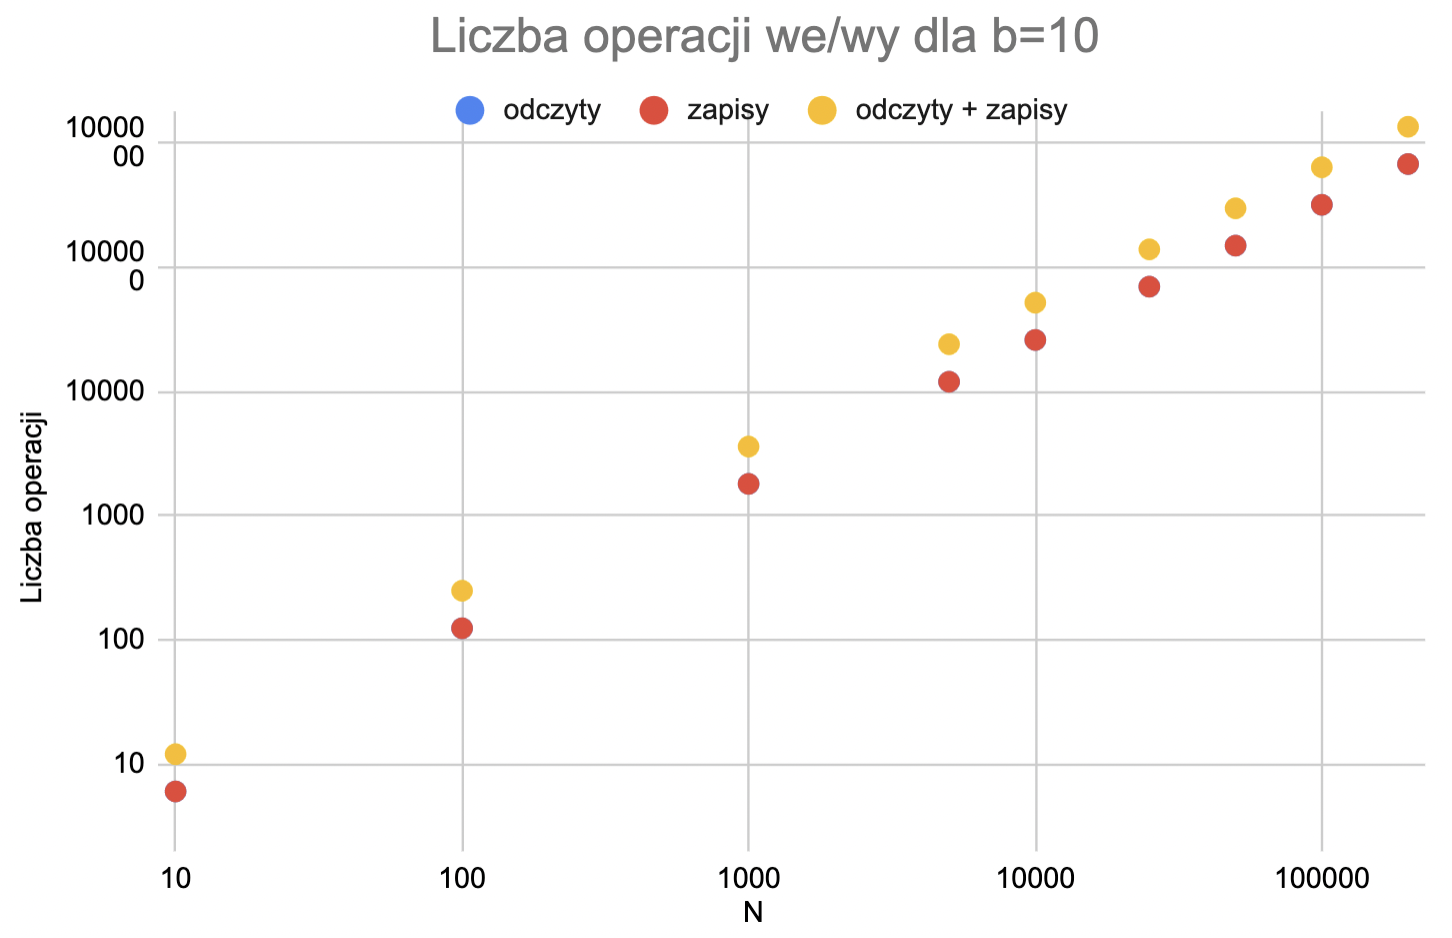
\includegraphics[width=10cm]{b10}
\end{center}
Przy losowaniu rekordów otrzymujemy w średnim przypadku $N/2$ serii, co widać  po wylosowanych danych.
Powyższe wyniki są zgodne z rozważaniami teoretycznymi mimo drobnych odstępstw, które
związane są ze szczegółami implementacyjnymi (np. pewnymi nadmiarowymi odczytami/zapisami).  Pragnę zauważyć również, że teoretyczna liczba faz odpowiada zmierzonej (poza przypadkami, w których \textbf{złączyły
się dwie lub więcej serii} tak jak np.  dla $N=10$ czy $N=1000$).   Ilość zapisów i odczytów jest taka sama w każdym z przypadków (kropki zapisów i odczytów pokrywają się na wykresie).
\\\\ Otrzymaliśmy zależność  "liniową" w skali 
logarytmicznej na obu osiach.  W rzeczywistości w średnim przypadku punktów nie łączy prosta,  bo 
\begin{gather*}
	log(T_{\text{Avg}}) = log(\frac{4N\ceil{log_2(N) - 1}}{b}) =  log(4) + log(N) + log(\ceil{log_2(N) - 1}) - log(b)
\end{gather*}
czyli dla $K = log(N)$
\begin{gather*}
	log(T_{\text{Avg}}) = K + log(4) - log(b) + log(\ceil{\frac{K}{log2} - 1})
\end{gather*} 
ale jako, że składnik $log(\ceil{\frac{K}{log2} - 1})$ jest bardzo mały, rozsądnym jest przybliżenie prostą
\begin{gather*}
	log(T_{\text{Avg}}) \approx K + log(4) - log(b)
\end{gather*}\\\\
dla $b=100$
\begin{center}
\begin{tabular}{ c c | c c c c | c c}
 N & liczba serii &odczyty & zapisy & r+w & liczba faz & teoretyczne r+w & teoretyczna liczba faz\\ 
\hline
 10 & 5 & 6 & 6 & 12 & 2 & 1.2 & 3\\  
 100 & 54 & 18 & 18 & 36 & 6 & 24 & 6 \\
 1000 & 504 & 189 & 189 & 378 & 9 & 4000 & 10\\
 5000 & 2481 & 1211 & 1211 & 2422 & 12 & 2400 & 12\\
 10000 & 4925 & 2612 & 2612 & 5224 & 13 & 5200 & 13 \\
 25000 & 12464 &  7013 & 7013 & 14026 & 14 & 14000 & 14 \\
 50000 & 24932 & 15013 & 15013 & 30026 & 15 & 30000 & 15\\
 100000 & 49875 & 32016 & 32016 & 64032 & 16 & 64000 & 16\\
 200000 & 100218 & 68017 & 68017 & 136034 & 17 & 136000 & 17\\
\end{tabular}
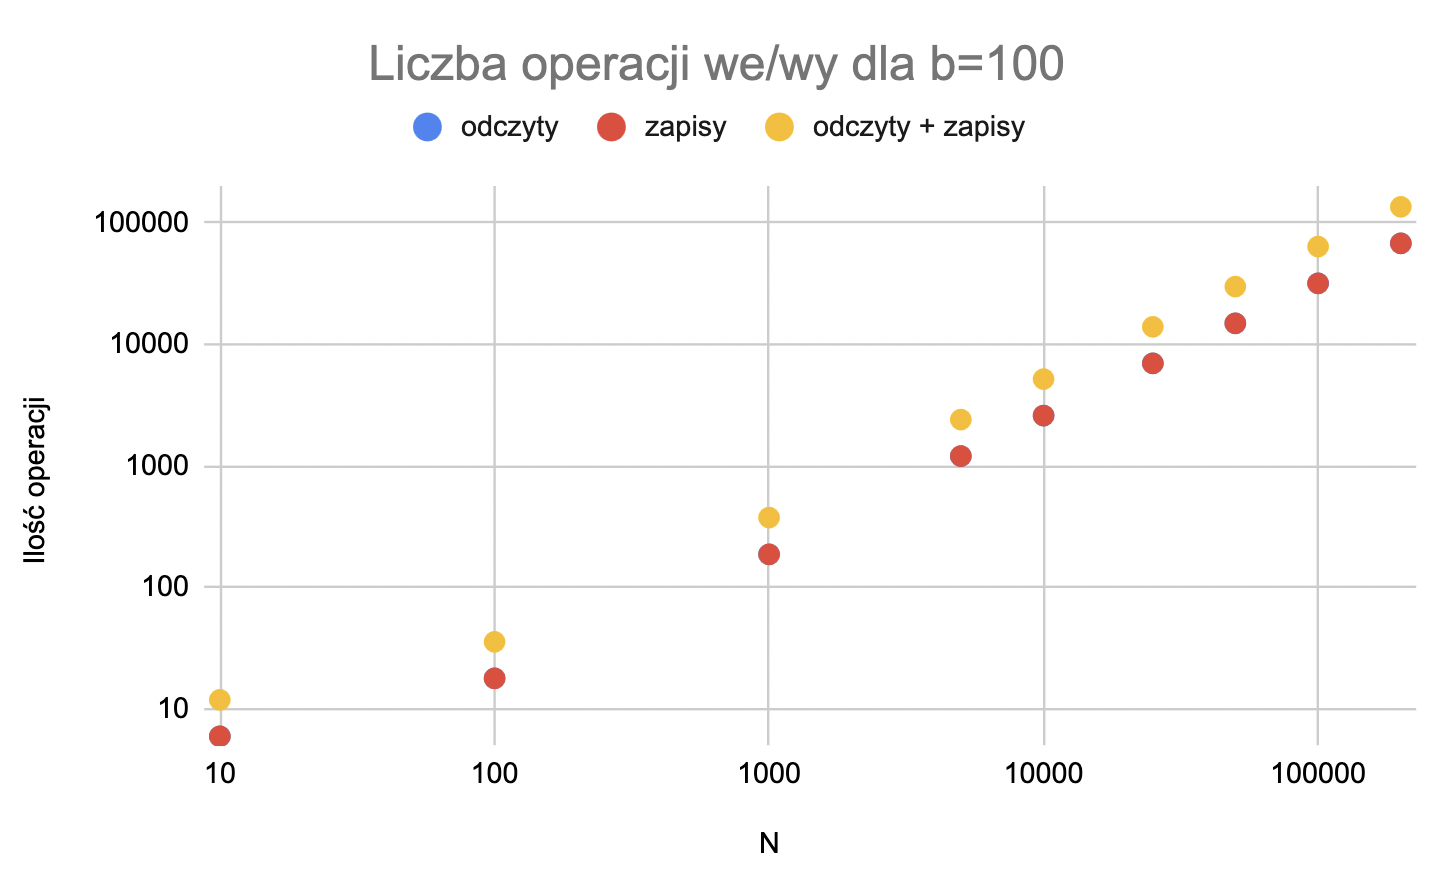
\includegraphics[width=10cm]{b100}
\end{center}
Jak widać \textbf{liczba faz w zależności od 
$N$ nie jest różna dla różnych współczynników blokowania} - zgodnie ze wzorem zależy tylko od ilości serii.
\begin{center}
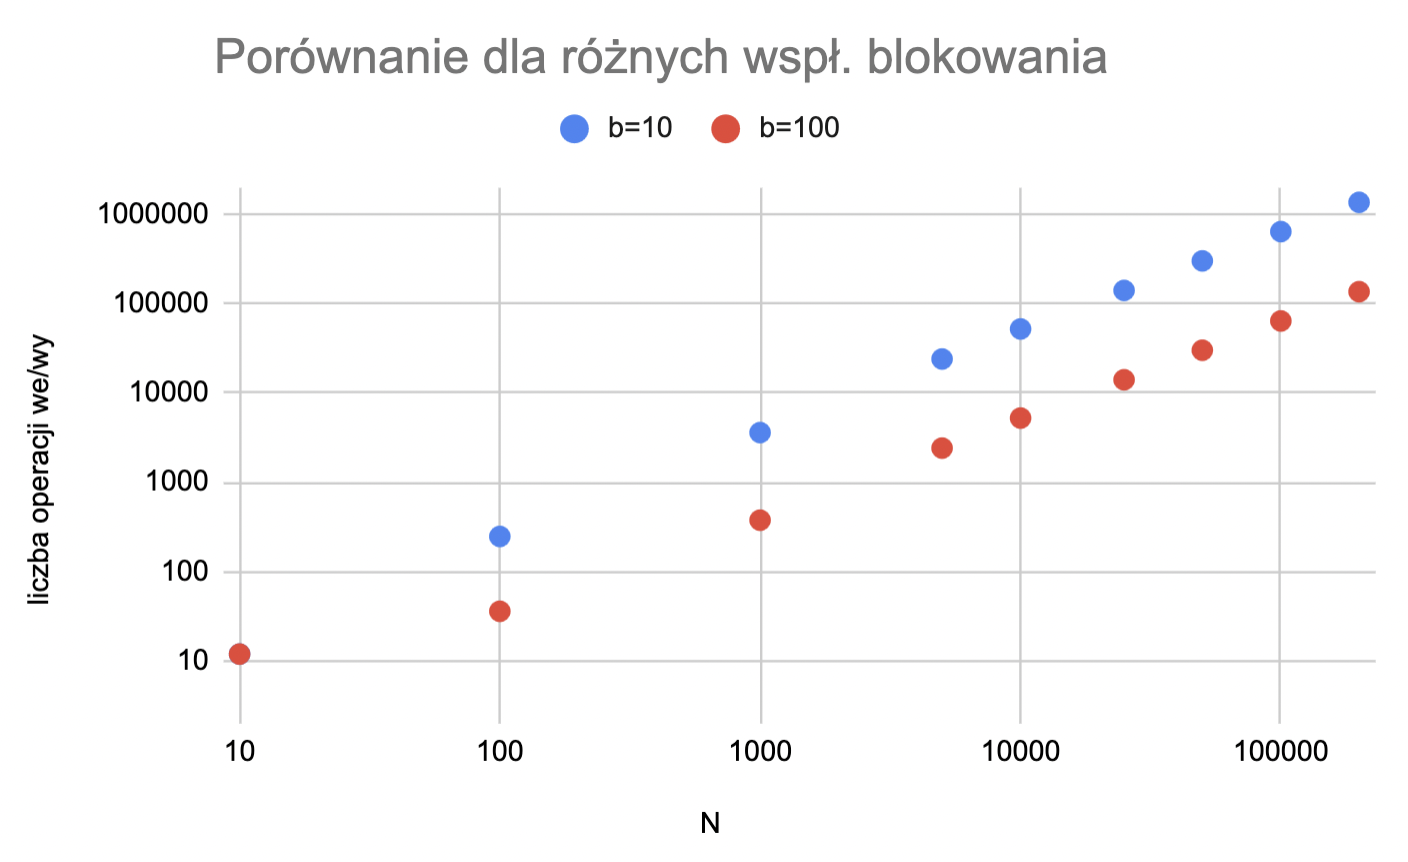
\includegraphics[width=10cm]{b}
\end{center}
Różni się natomiast liczba operacji wejścia-wyjścia, \textbf{zgodnie z intuicją czym większa
strona tym rzadziej ją wymieniamy} (spadek liniowy względem $\frac{1}{b}$, czyli jak widać na wykresie o jeden rząd wielkości mniej, bo $\frac{b_2}{b_1} = 10$). Dla małej ilości rekordów ($N=10$) nie ma różnicy spowodowanej
rozmiarem bloków, ponieważ w obu przypadkach \textbf{zostanie użyta tylko jedna strona} (pokrywające się 
kropki na wykresie - pierwsza czerwona kropka od lewej).
\section{Podsumowanie}
Projekt pozwolił na zapoznanie się z algorytmem sortowania przez scalanie plików sekwencyjnych i dał 
wgląd na mechanizm blokowego zapisu danych na dysku. \textbf{Wyniki eksperymentu można uznać za zgodne z oczekiwaniami} pomimo drobnych różnic spowodowanych \textbf{szczegółami implementacyjnymi oraz losowym
łączeniem się serii}.  Liczba operacji i/o zwiększa się proporcjonalnie do zmniejszania współczynnika blokowania, natomiast współczynnik ten nie ma wpływu na ilość faz algorytmu.  W końcu, dla rekordów w ilości 
mniejszej od obu rozmiarów stron  nie ma różnic w działaniu alogorytmów dla różnych wspł.  blokowania.



\end{document}
